\section{Conceptos Fundamentales}

\subsection{RISC-V}

RISC-V es un \ac{ISA} abierta y libre de \textit{royalties}, desarrollada originalmente en la Universidad de Berkeley. Desde sus inicios en 2010, ha sido diseñada para permitir implementaciones ligeras, de bajo consumo y fácilmente adaptables para diversos dispositivos. Además, su flexibilidad, bajo costo y capacidad de personalización lo posicionan como un serio competidor frente a arquitecturas más tradicionales como ARM, con el principal objetivo de desbancarlo en términos de rendimiento y consumo, siendo precisamente éstos los más importantes para el proyecto actualmente. Si bien es posible, gracias a la capacidad de modularización, estar presente en diferentes escenarios, RISC-V tiene su mayor relevancia en sistemas embebidos y sensores \ac{IoT}, estimándose que miles de millones de unidades equipadas con RISC-V ya están en circulación \cite{riscvInfo}.

RISC-V potencia la colaboración e innovación al ser una plataforma abierta que no requiere revelar propiedad intelectual, lo cual permitiría a, por ejemplo, Europa, a diseñar sus propios procesadores sin depender de terceros, siendo prueba de ello la fuerte inversión que está realizando en potenciar esta industria \cite{europaRISCV}. De hecho, fruto de esta inversión es precisamente este programa de máster, enmarcado en el programa PERTE-CHIP \cite{perteChip}. Un ejemplo de procesador RISC-V se presenta en \ref{fig:fotoChip}.

\begin{figure}[!ht]
  \centering
  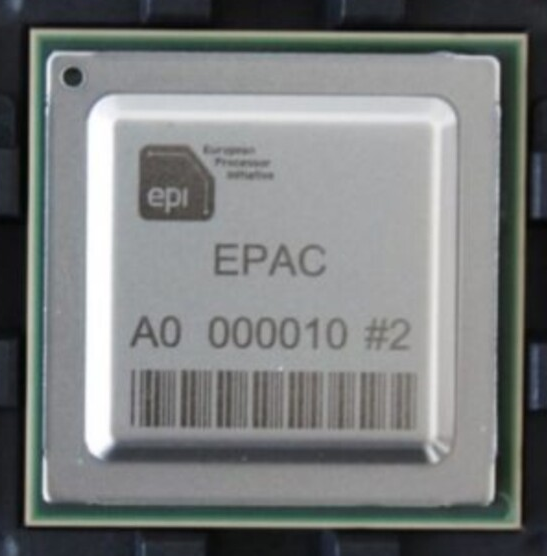
\includegraphics[width=4.5cm]{figures/chip.png}
  \caption{El primer chip RISC-V europeo, EPAC. Fuente: \cite{chipFoto}}
  \label{fig:fotoChip}
\end{figure}

\subsection{Cola FIFO}
\label{st:colasFifo}
Una cola \ac{FIFO} es una estructura de datos en la que el primer elemento que entra es el primero que sale, siguiendo el principio de una fila en la vida real. En hardware, las colas FIFO suelen implementarse como bloques de memoria con dos punteros (lectura y escritura) y lógica de control que garantiza que los datos se lean en el mismo orden en que fueron escritos. En el diseño digital, las FIFO se usan como \textit{buffers} entre módulos que operan a velocidades o relojes diferentes, o para absorber variaciones en el flujo de datos. Pueden ser síncronas (un solo dominio de reloj) o asíncronas (diferentes dominios de reloj en lectura y escritura, con circuitos de sincronización). En el contexto de este trabajo, las FIFO utilizadas son de carácter síncrono, a modo de simplificar el diseño final.

Las colas FIFO presentan un considerable número de ventajas, destacando:

\begin{enumerate}
    \item Aislamiento entre productores y consumidores
    \item Simplificación de la lógica de control
    \item Facilidad para integrarse en arquitecturas \textit{pipeline}
    \item Versatilidad en IP cores
    \item Evitan pérdidas de datos, sirviendo de almacenamiento temporal
\end{enumerate}

\subsection{FPGA}

Los \ac{FPGA} surgieron en la década de 1980 como una solución intermedia entre circuitos integrados de propósito general y los \ac{ASIC}, chips de propósito específico, con el objetivo de tener una plataforma con capacidad suficiente para desplegar prototipos \textit{hardware} y agilizar los procesos de desarrollo. Fue precisamente la empresa Xilinx, actualmente AMD, la que introdujo en 1985 el primer FPGA comercial, permitiendo a los diseñadores configurar y reconfigurar la lógica interna del chip un número casi ilimitado de veces, perfecto para pruebas \cite{historiaFPGA}. En la actualidad, los FPGAs han pasado de ser componentes para lógica reconfigurable a \ac{ACAP}s \cite{amdACAP}, plataformas heterogéneas de aceleración que integran bloques de CPU, motores para \ac{IA} y \ac{DSP}, memoria de alta velocidad y conectividad coherente. Además, la adopción en la nube y el empuje por herramientas (propietarias y open-source), los ponen como opción clave para aceleración en centros de datos y computación en el \textit{edge}. En este contexto, destaca Vivado Design Suite \cite{vivadoInfo}, la herramienta de desarrollo empleada en este trabajo.

Los retos actuales incluyen la reducción de la complejidad del flujo de diseño, el desarrollo de estándares abiertos para operar entre plataformas de fabricantes distintos, y el equilibrio entre programabilidad y rendimiento. A pesar de que el uso de lenguajes de alto nivel gracias a la adopción del \ac{HLS} ha simplificado el desarrollo, todavía existe una curva de aprendizaje pronunciada. En el futuro, se espera que los FPGA integren cada vez más interfaces coherentes como CXL, se adapten mejor a los flujos de trabajo de IA y expandan su papel en computación en el \textit{edge} y aplicaciones de carácter científico. En la figura \ref{fig:fpgaNexys} puede verse la placa FPGA Nexys A7, de Diligent, empleada a lo largo del máster.

\begin{figure}[!ht]
  \centering
  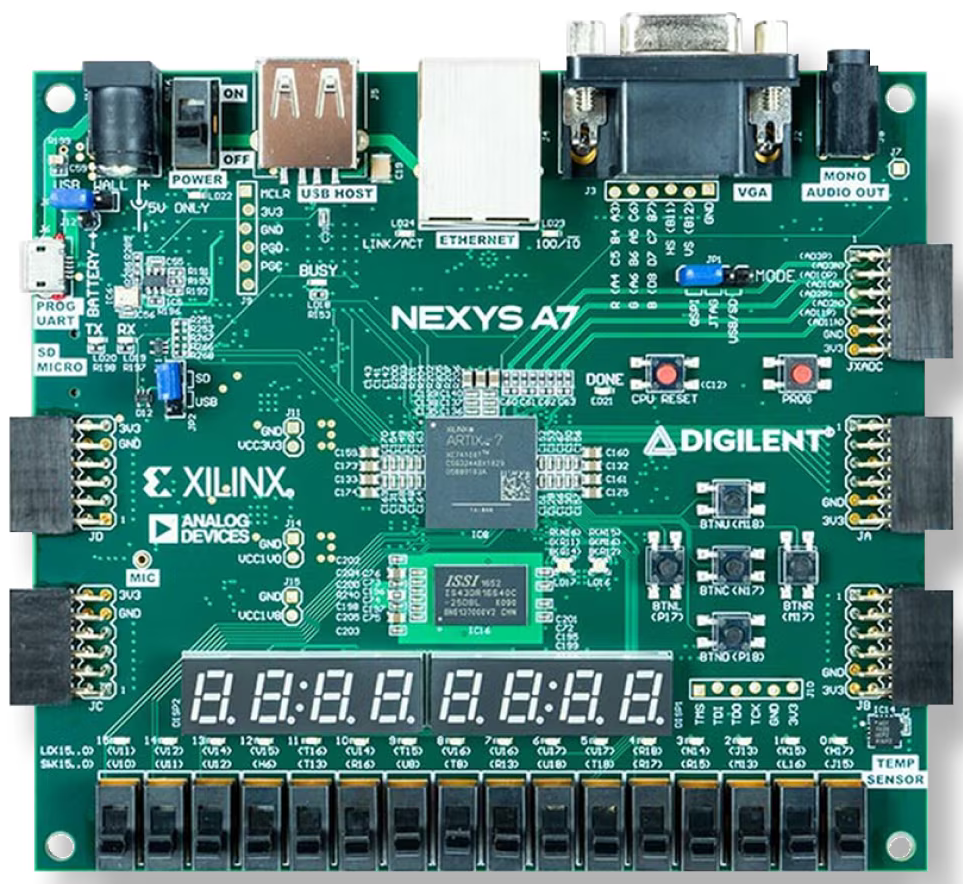
\includegraphics[width=6.5cm]{figures/nexysFoto.png}
  \caption{Diligent Nexys A7. Fuente: \cite{nexysFoto}}
  \label{fig:fpgaNexys}
\end{figure}

\subsection{Diseño \textit{hardware}}

Es el proceso de concebir, describir y realizar un sistema directamente en términos de sus componentes físicos y su comportamiento electrónico, sin abstraerse totalmente al software o a un nivel puramente algorítmico \cite{disenoHW}, lo que implica definir cómo estará estructurado y cómo funcionará el circuito que implemente la funcionalidad deseada.

\subsubsection{Diferencias con el diseño \textit{software}}

A diferencia del diseño \textit{software}, el diseño \textit{hardware} no trata de escribir un programa que un procesador interpretará, sino de definir el propio procesador y/o el circuito que ejecutará una tarea planteada. Una comparativa puede verse en \ref{tbl:compHWSW}.

\begin{table}[H]
\centering
\caption{Comparación entre diseño a nivel de hardware y diseño a nivel de software}
\begin{tabular}{|p{4cm}|p{5.5cm}|p{5.5cm}|}
\hline
\textbf{Aspecto} & \textbf{Diseño a nivel de hardware} & \textbf{Diseño a nivel de software} \\ \hline
\textbf{Descripción} & Definición de la funcionalidad de un sistema mediante componentes físicos y lógica digital. & Definición de instrucciones y algoritmos que serán ejecutados por un procesador o máquina virtual. \\ \hline
\textbf{Lenguajes} & HDL (VHDL, Verilog, SystemVerilog) y herramientas de síntesis/implementación. & Lenguajes de alto o medio nivel (C, C++, Python, Java, etc.). \\ \hline
\textbf{Unidad de trabajo} & Señales, registros, puertas lógicas, bloques IP, rutas de datos, temporización. & Variables, estructuras de datos, funciones, hilos, procesos. \\ \hline
\textbf{Ejecución} & El comportamiento está “fijo” en el hardware (aunque pueda ser reconfigurable en FPGA). & Se ejecuta secuencial o concurrentemente sobre hardware ya existente. \\ \hline
\textbf{Paralelismo} & Intrínseco: múltiples operaciones ocurren en paralelo por diseño físico. & Generalmente limitado al paralelismo gestionado por hilos/procesos del software. \\ \hline
\textbf{Tiempo de desarrollo} & Mayor complejidad y validación más costosa, incluye simulación, síntesis, implementación y pruebas en hardware real. & Más rápido de iterar y depurar; la validación se hace en un entorno controlado (IDE, simuladores de software). \\ \hline
\textbf{Optimización} & Área, consumo de energía, latencia y frecuencia de operación. & Tiempo de ejecución, uso de memoria, escalabilidad del código. \\ \hline
\end{tabular}
\label{tbl:compHWSW}
\end{table}

\subsubsection{Principales puntos de vista}

Los principales puntos de vista del diseño a nivel \textit{hardware} son los siguientes:

\begin{itemize}
    \item \textbf{Diseño lógico}: descripción del comportamiento con HDLs como VHDL o Verilog, especificando registros, puertas lógicas, \ac{FSM}s, y protocolos de interconexión a utilizar.
    
    \item \textbf{Diseño estructural}: organización y conexionado de los módulos o IPs del diseño, integrándolos en FPGAs, ASICs o dispositivos similares mediante el uso de líneas de comunicación y/o protocolos de interconexión planteados en el diseño lógico.
    
    \item \textbf{Diseño físico}: es la fase del diseño donde se implementa el diseño de forma física en el silicio, incluyendo ubicación de los módulos/IPs, enrutado de las conexiones y optimizaciones de área y consumo.
    
    \item \textbf{Diseño eléctrico}: definición de niveles de voltaje y limitaciones de corriente máxima dentro del circuito, comprobaciones temporales de las señales y su estabilidad, así como compatibilidad con los buses/protocolos de interconexión utilizados.
\end{itemize}

\subsubsection{Conceptos clave}

\begin{adjustwidth}{1.5cm}{}
\textbf{Metodología EDA} \vspace{0.25cm} \\
A grandes rasgos, pueden verse dos tipos principales de metodologías: las de gestión de proyectos, y las técnicas, centradas en la optimización del producto final. Será precisamente en ésta última categoía donde entran las metodologías del diseño de \textit{hardware}. En este contexto, se entiende por \emph{metodología técnica} al conjunto de enfoques, procedimientos y herramientas utilizadas para diseñar, desarrollar, verificar y optimizar un producto desde el punto de vista técnico o ingenieril. \cite{metodologiasHW}. En este contexto, se emplean metodologías variadas, como \textit{Top-Down}, que descompone el sistema en módulos jerárquicos hasta llegar a los módulos básicos, y \textit{Bottom-Up}, que consiste en construir el sistema a partir de módulos básicos hasta llegar a abarcar completamente el sistema a desarrollar. 

Sin embargo, la metodología relevante dentro de este proyecto es la basada en herramientas \ac{EDA}, siendo la metodología base para las herramientas utilizadas en este trabajo, como es la Vivado Design Suite, ya mencionada. Esta metodología adopta un enfoque estructurado e iterativo que se extiende desde la definición de requisitos hasta la fabricación física. El flujo de la metodología EDA se basa en dos grandes bloques: Front-End y Back-End, con verificación continua en todas las etapas. \cite{metodologiaFernando}. Este flujo se detalla en \ref{tbl:flujoEDA}.

\begin{table}[!ht]
\centering
\begin{tabular}{|l|p{9cm}|}
\hline
\textbf{Etapa} & \textbf{Sub-etapas} \\ \hline
Especificación y planificación & Requisitos funcionales y no funcionales; Arquitectura y selección de IP cores; Modelado de alto nivel: SystemC, Matlab \\ \hline
Front-End & Diseño algorítmico y HLS; Diseño lógico RTL: Verilog, VHDL, SystemVerilog; Reutilización de IP (Soft y Hard); Síntesis lógica a netlist \\ \hline
Back-End & Planificación física, placement y routing; Síntesis y distribución de reloj; Verificación física: DRC y LVS \\ \hline
Verificación & Funcional y formal; Análisis de tiempo estático; Simulación post-layout \\ \hline
Sign-off y fabricación & Validaciones finales y análisis de consumo; Generación de vectores de test (DFT, BIST); Creación de archivos GDSII y tape-out \\ \hline
\end{tabular}
\caption{Resumen de las actividades en cada etapa del flujo de la metodología EDA}
\label{tbl:flujoEDA}
\end{table}

Gracias a esta metodología, el diseño de ASICs y sistemas complejos integra fases iterativas, reutilización de IPs, modelado jerárquico y verificación exhaustiva, buscando optimizar coste, tiempo y fiabilidad. 
\end{adjustwidth}

\vspace{0.4em} % Espacio vertical entre párrafos

\begin{adjustwidth}{1.5cm}{}
\textbf{Front-end y Back-end} \vspace{0.25cm} \\
El Front-End se refiere a la fase inicial de planteamiento del diseño \textit{hardware}, centrada en la funcionalidad y la lógica del circuito, antes de realizar implementación física alguna. Por otra parte, el Back-end va después del Front-end, y se centra en la implementación física del diseño planteado y en preparar el circuito para la fabricación en silicio \cite{metodologiaFernando}. En \ref{tbl:frontBack} se presentan detalladamente las principales actividades de estas dos fases.

\begin{table}[h!]
\centering
\begin{tabular}{|l|p{9cm}|}
\hline
\textbf{Etapa} & \textbf{Descripción} \\ \hline
\multicolumn{2}{|c|}{\textbf{Front-End}} \\ \hline
Diseño algorítmico & Modelado funcional de los bloques o sistema completo sin preocuparse por la implementación física (ej. algoritmos en SystemC o Matlab). \\ \hline
Síntesis de alto nivel (HLS) & Traducción de modelos funcionales a RTL considerando restricciones de frecuencia, área y consumo. \\ \hline
Diseño lógico RTL & Descripción detallada de la lógica interna, rutas de datos y control usando Verilog, VHDL o SystemVerilog, lista para síntesis. \\ \hline
Reutilización de IP & Integración de bloques ya diseñados: Soft IP (modificable, en RTL) o Hard IP (cercano a silicio, optimizado). \\ \hline
Síntesis lógica & Conversión final de RTL a netlist de puertas lógicas adaptada a la tecnología seleccionada. \\ \hline
\multicolumn{2}{|c|}{\textbf{Back-End}} \\ \hline
Planificación física & Distribución de bloques y componentes en el chip para optimizar área y conexiones. \\ \hline
Placement & Ubicación óptima de celdas para minimizar retardos y conexiones. \\ \hline
Routing & Trazado de interconexiones físicas de celdas en el chip o configuración de recursos en FPGA. \\ \hline
Síntesis y distribución de reloj & Creación de la red de sincronización para que todos los bloques funcionen coordinadamente. \\ \hline
Verificación física & Comprobación de reglas de diseño (DRC) y equivalencia entre esquemático y layout (LVS). \\ \hline
\end{tabular}
\caption{Resumen de etapas del Front-End y Back-End en diseño digital}
\label{tbl:frontBack}
\end{table}
\end{adjustwidth}

\vspace{0.4em} % Espacio vertical entre párrafos

\begin{adjustwidth}{1.5cm}{}
\textbf{Hardware Description Language (HDL)} \vspace{0.25cm} \\
Los \ac{HDL}s son lenguajes de programación especializados utilizados para describir, modelar y simular el comportamiento y la estructura de circuitos electrónicos digitales. A diferencia de los lenguajes de programación tradicionales (como C o Python), los HDLs permiten especificar tanto el comportamiento lógico como la implementación física de un sistema, posibilitando su síntesis en dispositivos de hardware como FPGAs o ASICs. Su aparición en la segunda mitad del siglo XX revolucionó la forma en que ingenieros y diseñadores desarrollan hardware, permitiendo ciclos de diseño más rápidos y complejos. \cite{infoHDL}. Entre los HDLs más conocidos se encuentran VHDL, Verilog y Chisel. De todos ellos, el más representativo en el contexto de este trabajo es Verilog, el cual será detallado en posteriores apartados.
\end{adjustwidth}


\vspace{0.4em} % Espacio vertical entre párrafos

\begin{adjustwidth}{1.5cm}{}
\textbf{Hardware Level Synthesis (HLS)} \vspace{0.25cm} \\
\ac{HLS}, también conocido como \emph{behavioral synthesis} o \textit{algorithmic synthesis}, es un proceso automatizado que transforma una descripción funcional de alto nivel, como escrita en C, C++, SystemC, MATLAB o similar en una representación de hardware en HDLs como Verilog \cite{infoHLS}

A la hora de diseñar \textit{hardware} para probar en FPGAs, HLS ofrece ventajas como un desarrollo más rápido, una mayor abstracción y portabilidad entre plataformas. Permite a los diseñadores trabajar con lenguajes de alto nivel como C o C++, algo especialmente interesante para diseñadores de \textit{software}. La depuración del código generado por HLS puede ser un desafío y la calidad de salida de la herramienta depende de la experiencia del diseñador, el cual, para alcanzar una mayor optimización del diseño generado, deberá revisar la generación obtenida. \cite{ventajasHLS}
\end{adjustwidth}

\vspace{0.4em} % Espacio vertical entre párrafos

\begin{adjustwidth}{1.5cm}{}
\textbf{Las señales Clock y Reset} \vspace{0.25cm} \\
En procesadores, microcontroladores o circuitos implementados en FPGA, las señales Clock y Reset son fundamentales para que el hardware funcione de manera ordenada y predecible.

La señal de \emph{Clock} (reloj) es una onda periódica, normalmente cuadrática, que marca el ritmo al que un circuito digital ejecuta operaciones. \cite{weste2015cmos} \cite{harris2021digital}. Su principal función es sincronizar el funcionamiento de todos los módulos donde esté conectada, como flip-flops, registros y contadores, de manera que los cambios de estado ocurran únicamente en momentos definidos, normalmente en los bordes de subida (\textit{active-high}) o bajada (\textit{active-low}) de la señal. Asimismo, el término  \emph{frecuencia de clock}, se refiere a la velocidad con las que se producen estas subidas y bajadas de la señal, siendo a mayor frecuencia, mayor el número de transiciones por unidad de tiempo, lo que desemboca en una mayor capacidad de procesamiento, mientras que su ciclo de trabajo y estabilidad en las transiciones de subida y bajada influyen en la fiabilidad de las operaciones de los módulos conectados a dicha señal. 

Por otro lado, La señal de \emph{Reset} tiene la función de inicializar el sistema a un estado conocido y seguro \cite{resetTechniques}. Al activarse, fuerza a todos los registros y elementos secuenciales a tomar valores iniciales, garantizando que el sistema comience siempre en condiciones predecibles. Existen dos tipos principales: el reset síncrono, que actúa junto con el clock, y el reset asíncrono, que se activa inmediatamente sin esperar un ciclo de reloj. Esta señal es crucial al encender un dispositivo, para evitar estados indeterminados, y también se utiliza para reiniciar el sistema en caso de errores o bloqueos.

La importancia conjunta de ambas señales es clara: el \textit{clock} determina cuándo ocurren las acciones dentro del hardware, mientras que el \textit{reset} define desde dónde y en qué condiciones se empieza a trabajar. Sin un clock estable, el sistema pierde el orden en sus operaciones; sin un reset confiable, el arranque puede ser inestable, por tanto, poco seguro, lo que podría desembocar en graves accidentes allá donde esté desplegado el circuito en cuestión.
\end{adjustwidth}

\vspace{0.4em} % Espacio vertical entre párrafos

\begin{adjustwidth}{1.5cm}{}
\textbf{Módulo RTL y módulo IP} \vspace{0.25cm} \\
Un módulo \ac{RTL} es un bloque de hardware descrito en un lenguaje de descripción de hardware como Verilog, del cual se hablará posteriormente, y donde se especifica el comportamiento y la estructura del circuito a nivel de registros, señales y operaciones lógicas. El diseñador puede escribir este código manualmente o generarlo con herramientas automatizadas, y normalmente se tiene acceso al código fuente, lo que permite modificarlo, optimizarlo o adaptarlo a distintas plataformas. Un módulo RTL describe con detalle cómo funciona internamente el hardware y es portable. Por tanto, el módulo RTL se centra en el diseño detallado y editable del hardware. \cite{moduloRTL}

Por otro lado, un módulo \ac{IP} es un bloque de hardware ya diseñado, probado y empaquetado para ser reutilizado en múltiples proyectos. Generalmente es proporcionado por un fabricante o un tercero (por ejemplo, Xilinx o Intel/Altera) y puede venir como un diseño cerrado (\textit{black-box}) o con opciones limitadas de configuración. \cite{moduloIP}. Su uso suele ser más rápido porque evita diseñar el hardware desde cero, pero muchas veces no se puede ver ni modificar su implementación interna, ya que forma parte de la propiedad intelectual del proveedor. Por tanto, el módulo IP es una unidad reutilizable, e inmutable, que puede ser integrada en un diseño para agregarle funcionalidades. 

La diferencia principal entre ambos es que el módulo RTL es un diseño abierto y editable que describe el funcionamiento interno del hardware en detalle, de tipo \textit{white-box}, mientras que un módulo IP es un bloque ya terminado y optimizado que normalmente se usa como componente prefabricado, a menudo sin acceso a su código interno, pues, por norma general, está protegido por licencias.
\end{adjustwidth}

\vspace{0.4em} % Espacio vertical entre párrafos

\begin{adjustwidth}{1.5cm}{}
\textbf{Módulo Top} \vspace{0.25cm} \\
El módulo top (conocido también por \textit{top-level module}) es la unidad más elevada en la jerarquía de la arquitectura del sistema \textit{hardware} diseñado. Este módulo no es instanciado dentro de otro, y sirve como contenedor de todos los submódulos necesarios para materializar el diseño completo, actuando como el punto de integración final antes de su implementación física \cite{infoTop}. Es en el módulo Top donde se define y organiza la interfaz global con el exterior, como los pines I/O de un FPGA, a la vez que sincroniza la interconexión entre bloques internos que tiene instanciados.
\end{adjustwidth}

\vspace{0.4em} % Espacio vertical entre párrafos

\begin{adjustwidth}{1.5cm}{}
\textbf{Wrapper} \vspace{0.25cm} \\
Por otra parte, el \textit{wrapper} desempeña un rol igualmente crucial como intermediario entre un módulo RTL o IP ya existente con el resto del sistema. En plataformas como Vivado Design Suite, herramienta empleada en este trabajo, el \textit{wrapper} se genera para conectar los puertos de entrada y salida del diseño con los pines físicos definidos en el archivo de restricciones. Asimismo, el \textit{wrapper} también facilita la adaptación entre jerarquías, ajustes en nombres de señales o protocolos, y la integración de módulos que de otra forma serían incompatibles \cite{infoWrapper}. El uso de \textit{wrappers} permite mantener la integridad del módulo original (por ejemplo, un IP de terceros), mientras se ajusta a requerimientos externos sin modificar su código fuente. El objetivo general de un \textit{wrapper} es, en múltiples ocasiones, facilitar la conectividad exclusivamente, lo que hace que casi siempre estén carentes de lógica específica. 

Llegados a este punto, puede parecer que el módulo Top y un \textit{Wrapper} son muy parecidos. En realidad, desempeñan funciones complementarias. El primero constituye la instancia principal que integra el diseño, mientras que el segundo actúa como un mediador que permite integrar módulos de cualquier tipo, como IPs de terceros, los cuales, en numerosos casos, presentan especificaciones técnicas distintas respecto al resto del diseño. \cite{infoWrapper}.
\end{adjustwidth}

\vspace{0.4em} % Espacio vertical entre párrafos

\begin{adjustwidth}{1.5cm}{}
\textbf{Block Design} \vspace{0.25cm} \\
En el diseño de \textit{hardware} digital, el concepto de \emph{Block Design} se refiere a la construcción de sistemas a partir de bloques modulares que poseen funcionalidades concretas \cite{infoBlockDesign}. Cada bloque representa un módulo, que puede ser desde un procesador, un controlador de memoria, o un módulo personalizado. Estos bloques se conectan entre sí a través de interfaces, como el bus \ac{AXI}. 

Una de las principales ventajas del enfoque de Block Design es la modularidad, permitiéndose el reuso de IPs de terceros, así como módulos personalizados, dentro de un mismo desarrollo. De esta manera, no se necesita trabajar directamente a nivel de puertas lógicas o escribir RTL desde cero, basta con importar cada componente dentro del diseño y generar un \textit{wrapper} que contenga información de todos los presentes dentro del mismo. Así, se acelera el proceso de desarrollo y mejora la escalabilidad del diseño, permitiendo a la vez una visualización clara y jerárquica del sistema, útil para entender y depurar arquitecturas complejas \cite{infoBlockDesign} \cite{maxfield2004design}.

En la práctica, este método es ampliamente utilizado en el desarrollo \textit{hardware}. En el contexto de este trabajo, se ha realizado el desarrollo del diseño a nivel \textit{hardware} precisamente sobre un Block Design, por la buena integración y facilidad de uso dentro de Vivado Design Suite.En la figura \ref{fig:bdVivado} se presenta un ejemplo de Block Design realizado con Vivado Design Suite

\begin{figure}[!ht]
  \centering
  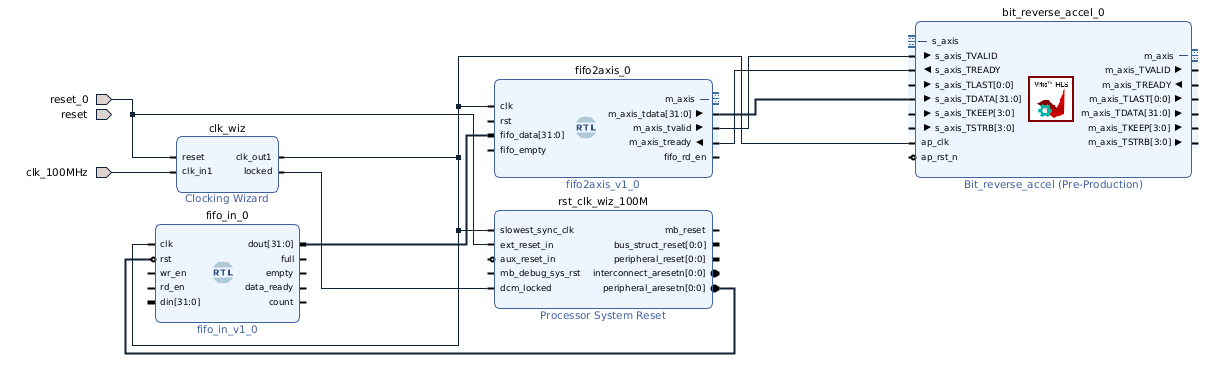
\includegraphics[width=11cm]{figures/vivadoBD.png}
  \caption{Block Design del diseño realizado en Vivado}
  \label{fig:bdVivado}
\end{figure}

\end{adjustwidth}

\begin{adjustwidth}{1.5cm}{}
\textbf{Testbench} \vspace{0.25cm} \\
En el diseño de circuitos digitales, un \emph{testbench} o banco de pruebas es un archivo escrito generalmente en lenguajes HDL como Verilog, y su función principal es aplicar estímulos al circuito bajo prueba, el \ac{DUT}, (o el \ac{UUT}, si se quiere probar un módulo y no el conjunto completo), para finalmente observar las respuestas que se producen, y así comprobar el cumplimiento de los requisitos. El testbench no es un módulo más del diseño; es una herramienta de simulación. Dentro de él, se generan señales de entrada, se definen patrones de prueba (como impulsos de reloj, valores de datos, resets, etc.) y se supervisan las salidas del DUT por medio de equivalencias con lo esperado y aserciones.

Existen distintos niveles de sofisticación en los testbenchs: desde versiones simples que solo aplican algunos vectores de entrada manualmente, hasta entornos más complejos con generación automática de estímulos, verificación dirigida por cobertura (coverage-driven verification), e incluso entornos basados en metodologías formales como UVM (Universal Verification Methodology). En el máster se ha trabajado con UVM, sin embargo, los testbenchs realizados no lo emplean principalmente por errores incomprensibles al intentar integrarlo en el testbench utilizado para las simulaciones en Vivado.
\end{adjustwidth}

\subsection{Herramientas utilizadas}

\subsubsection{X-HEEP}
\label{st:xheep}
\ac{X-HEEP} \cite{machetti2024xheep} \cite{xheepInfo} es una plataforma RISC-V \textit{open-source}, diseñada como microcontrolador configurable y extensible, desarrollada en SystemVerilog por el \ac{EPFL}. Su arquitectura permite personalización en niveles como \textit{cores}, periféricos, memorias y topologías para habilitar aceleradores especializados sin modificar el \ac{MCU} base. Además, soporta múltiples flujos de simulación para pruebas y verificación, destacando Verilator, así como despliegue físico en FPGAs y ASICs, dando resultado a implementaciones como HEEPocrates o X-TRELA \cite{xheepInfoASIC}. A modo de resumen, se puede decir que X-HEEP es una plataforma de prototipado y simulación a nivel de \ac{SoC} RISC-V con capacidad de ir desde simulación RTL hasta emulación en FPGA y implementación en ASIC. Sin embargo, aunque se ha hablado sobre X-HEEP, lo cierto es que, en realidad, se haá uso de un \textit{fork} de X-HEEP llamado GR-HEEP \cite{grheepInfo}, preparado para el uso de periféricos y aceleradores externos, como el desarrollado en este proyecto.

En lo que respecta a su arquitectura, el diseño modular de X-HEEP está dividido en distintos dominios de energía (CPU, periféricos, memoria, always-on), optimizando el consumo y permitiendo habilitar/deshabilitar componentes según necesidad. Emplea cores del OpenHW Group como CVE2, CV32E40P(X), todos RISC-V de 32 bits estilo Harvard y sin cache, ideales para escenarios ultra-low-power y RTOS integrados. \cite{xheepDocs}. En \ref{tbl:xheepArch} se presentan los principales dominios en detalle. Finalmente, en la figura \ref{fig:xheepArch} se presenta un diagrama de la arquitectura en cuestión.

\begin{table}[h!]
\centering
\caption{Dominios del SoC X-HEEP}
\label{tab:dominios_xheep_texto}
\begin{tabular}{|l|p{9cm}|}
\hline
\textbf{Dominio} & \textbf{Descripción resumida} \\ \hline
CPU Subsystem & Núcleos RISC-V OpenHW de 32 bits (CVE2, CV32E40P, CV32E40PX, CV32E40X), arquitectura Harvard sin caché, protocolo OBI, diseñados para bajo consumo y con capacidad de apagado completo o por clock-gating. \\ \hline
Memory Banks & Múltiples bancos de memoria independientes para instrucciones y datos, accesibles en paralelo sin conflictos, con control granular de energía mediante clock-gating, retención o apagado individual. \\ \hline
Peripheral Subsystem & Conjunto de periféricos generales (timer, PLIC, I2C, SPI, 24 GPIO) conectados por una única interfaz con decodificación interna, con posibilidad de apagado o reducción de consumo cuando están inactivos. \\ \hline
Always-On Peripherals & Periféricos e IPs críticos que permanecen activos todo el tiempo (controlador SoC, boot ROM, gestor de energía, fast interrupt, DMA, timer, UART, 2 SPI, 8 GPIO), sin aplicar técnicas de apagado de energía. \\ \hline
\end{tabular}
\label{tbl:xheepArch}
\end{table}

\begin{figure}[!ht]
  \centering
  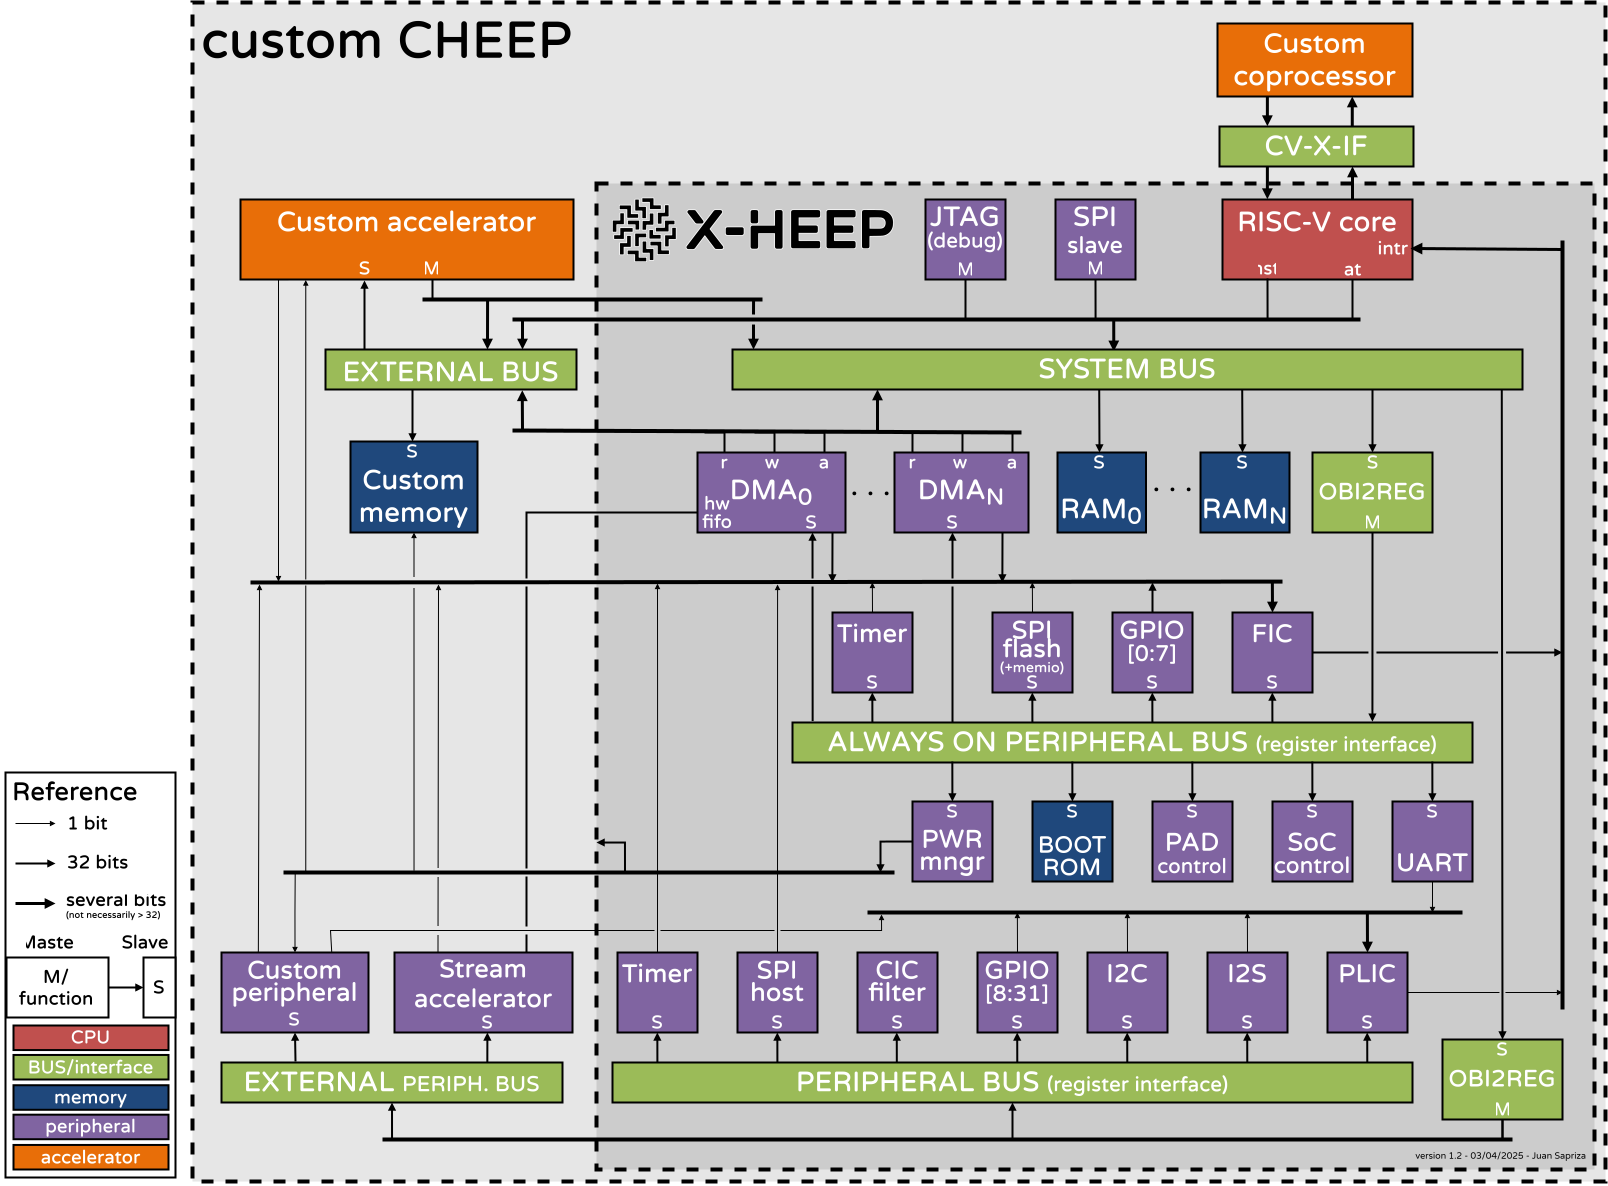
\includegraphics[width=11cm]{figures/xheepArch.png}
  \caption{Arquitectura de X-HEEP. Fuente: \cite{xheepInfo}}
  \label{fig:xheepArch}
\end{figure}



\subsubsection{Verilog}
Creado en 1984 por Phil Moorby y Prabhu Goel en Gateway Design Automation, su diseño buscaba una sintaxis familiar a programadores en C, lo que contribuyó a su rápida adopción. Fue estandarizado por primera vez como IEEE 1364-1995 (“Verilog-95”), seguido por revisiones en 2001 y 2005. En 2009, Verilog fue fusionado dentro de SystemVerilog bajo el estándar IEEE 1800-2009 y actualmente forma parte del estándar unificado IEEE 1800-2023. \cite{verilogEstandar}  Verilog ocupa un lugar central en el diseño digital moderno debido a su equilibrio entre legibilidad, flexibilidad y potencia. Fue originalmente un lenguaje propietario en los años 80, diseñado para modelado de hardware, y en la década de los 90 se abrió al dominio público a través de Open Verilog International (OVI), que lo llevó a estandarización del \ac{IEEE} \cite{verilogHistoria}. Su adopción global y la abundancia de herramientas de simulación y síntesis compatibles lo han consolidado como uno de los pilares del diseño digital moderno. En \ref{lst:verilogEjemplo} puede verse un ejemplo de un sumador desarrollado en Verilog.

\begin{lstlisting}[language=verilog,frame=single,caption={Código fuente en Verilog de un sumador},showstringspaces=false,label=lst:verilogEjemplo]
module adder_4bit(
    input  [3:0] a,
    input  [3:0] b,
    input        cin,
    output [3:0] sum,
    output       cout
);

    // Salidas del sumador
    assign {cout, sum} = a + b + cin;

endmodule
\end{lstlisting}

\subsubsection{FreeRTOS}
\label{st:freertos}
Antes de entrar en detalle con la herramienta FreeRTOS, es necesario explicar en qué consiste un \ac{RTOS}. Un RTOS es un tipo especializado de sistema operativo diseñado para gestionar tareas que deben ejecutarse dentro de límites de tiempo estrictos y predecibles. A diferencia de los sistemas operativos de propósito general, como Windows, que están orientados a la multitarea y la gestión eficiente de recursos, un RTOS se centra en garantizar que las tareas críticas se completen dentro de plazos específicos \cite{rtosInfo} \cite{rtosInfo_2}. 

Si bien hay multitud de opciones a día de hoy, destacan, entre otros, Zephyr \cite{zephyrInfo} y FreeRTOS \cite{freeRTOSInfo}, siendo este último el utilizado en el proyecto. Originalmente desarrollado por Richard Barry en 2003, y mantenido por Amazon desde 2017, FreeRTOS es un kernel de sistema operativo de tiempo real de código abierto, diseñado específicamente para sistemas embebidos con recursos limitados. Además, recientemente ha recibido soporte para RISC-V \cite{soporteRISCVFreeRTOS}. Las características principales de FreeRTOS son:

\begin{itemize}
    \item \textbf{Pequeño y eficiente}: diseñado para tener una huella de memoria mínima, lo que lo hace adecuado para microcontroladores con recursos limitados.
    \item \textbf{Multiplataforma}: compatible con más de 40 arquitecturas, incluyendo ARM, AVR, RISC-V, entre otras.
    \item \textbf{Planificación preemptiva}: implementa un planificador de tareas que permite la ejecución de tareas con prioridades, garantizando que las tareas críticas se ejecuten a tiempo.
    \item \textbf{Soporte para multitarea}: permite la crear y gestionar múltiples tareas, semáforos, colas y temporizadores, facilitando la programación concurrente.
    \item \textbf{Licencia MIT}: es de código abierto, lo que permite su uso y modificación sin restricciones.
\end{itemize}

Para finalizar la sección, se presenta en \ref{fig:logoFreeRTOS} el logo.

\begin{figure}[!ht]
  \centering
  
\includegraphics[width=6.5cm]{figures/Logo_freeRTOS.png}
  \caption{Logo de FreeRTOS. Fuente: \cite{freeRTOSLogo}}
  \label{fig:logoFreeRTOS}
\end{figure}


\subsubsection{Vivado Design Suite}
\label{st:vivado}
Vivado Design Suite \cite{vivadoInfo}, desarrollado originalmente por Xilinx en 2012, y ahora parte de AMD, es una plataforma integrada en la metodología basada en herramientas EDA. Sustituta del antiguo ISE Design Suite, fue creada desde cero para abordar las crecientes exigencias de diseño en FPGAs y SoCs modernos \cite{vivadoHistoria_1}. 

Vivado está construido sobre un modelo de datos compartido y escalable, que permite una integración fluida entre diseño, síntesis, análisis, simulación, depuración y cierre de tiempos (\textit{timing closure}) Su arquitectura favorece la visibilidad continua de métricas clave como utilización de recursos, potencia, congestión o tiempos, en todas las etapas del flujo de diseño. \cite{vivadoRazones}. Será, por tanto, Vivado Design Suite la empleada para la realización del diseño \textit{hardware} desarrollado en este trabajo.

Las principales herramientas presentes en Vivado Design Suite son:

\begin{itemize}
    \item \textbf{Vivado IDE}: Interfaz gráfica principal para capturar el diseño, gestionar proyectos, correr síntesis, implementación y generar el bitstream. Incluye consola Tcl para automatización y scripting.
    \item \textbf{Vivado Synthesis}: Motor de síntesis lógica para VHDL, Verilog y SystemVerilog, que convierte el código HDL en una netlist optimizada para la FPGA.
    \item \textbf{Vivado Implementation}: Realiza place \& route, optimiza para timing closure y genera el bitstream final del diseño.
    \item \textbf{Vivado Simulator (XSim)}: Simulador HDL integrado y multilenguaje para depurar el diseño antes de implementarlo en hardware.
    \item \textbf{Vivado IP Integrator}: Entorno gráfico para ensamblar IPs predefinidos y crear subsistemas usando interfaces como AXI de forma automática.
    \item \textbf{Vivado High-Level Synthesis (HLS)}: Herramienta para diseñar en C, C++ o SystemC y generar hardware a partir de código de alto nivel.
    \item \textbf{Vivado Logic Analyzer}: Permite la depuración en hardware mediante analizadores lógicos integrados (ILA) y monitorización de señales internas en tiempo real.
    \item \textbf{Vivado Power Analysis}: Estimación y análisis de consumo de potencia del diseño en distintas fases del flujo.
    \item \textbf{Vivado ECO Editor}: Permite aplicar Engineering Change Orders al diseño implementado sin necesidad de recompilar todo.
\end{itemize}

Para finalizar, se presenta en \ref{fig:proyectoVivado} un proyecto abierto en Vivado Design Suite.

\begin{figure}[!ht]
  \centering
  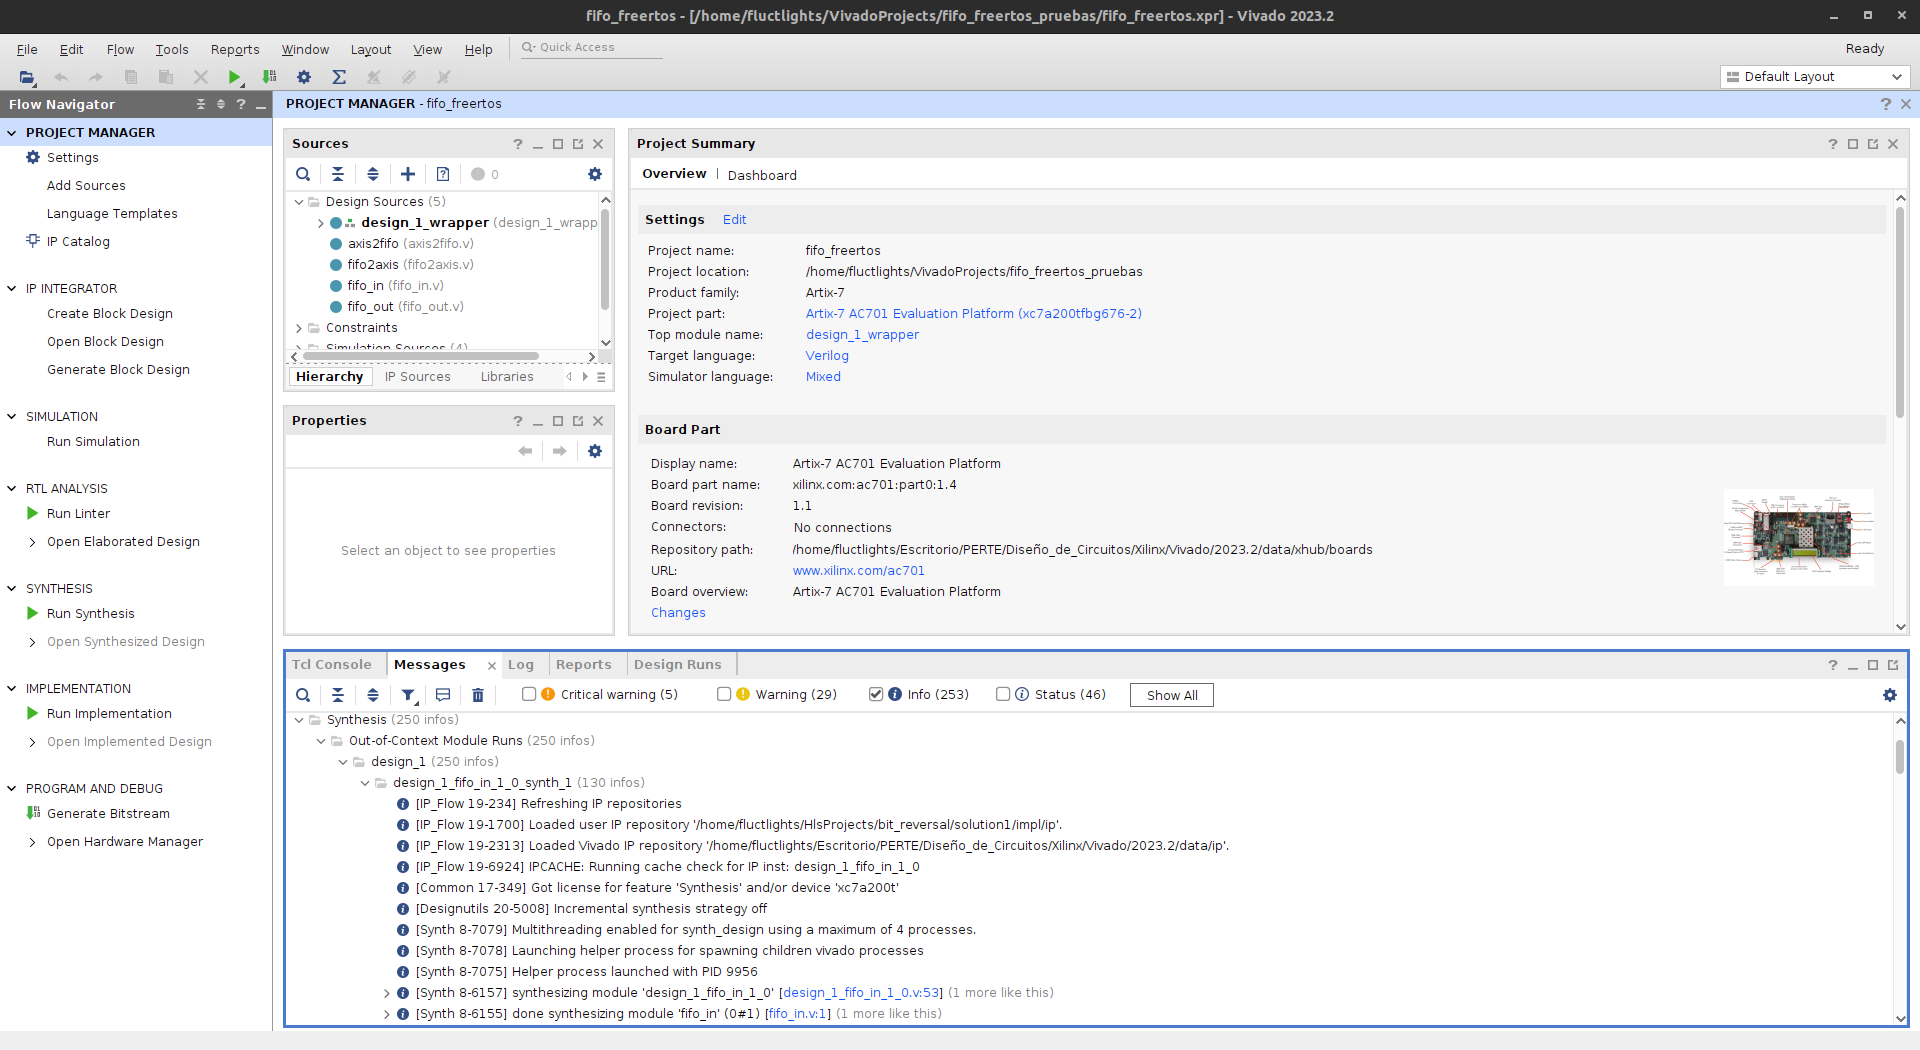
\includegraphics[width=11cm]{figures/proyectoVivado.png}
  \caption{Proyecto abierto}
  \label{fig:proyectoVivado}
\end{figure}

\subsubsection{Vitis HLS}
Vitis \ac{HLS} es una herramienta de síntesis de alto nivel desarrollada por Xilinx (ahora propiedad de AMD) que permite la conversión de código en C/C++ a RTL sintetizable para dispositivos FPGAs \cite{vitisHLSInfo} Esta herramienta facilita la creación de algoritmos complejos para \textit{hardware} sin necesidad de escribir código a lenguajes de descripción de \textit{hardware} tradicionales como VHDL o Verilog. Una de las principales ventajas de Vitis HLS es su capacidad para abstraer el diseño de hardware, permitiendo a los diseñadores centrarse en la funcionalidad del algoritmo en lugar de los detalles de implementación del hardware. La herramienta soporta directivas de síntesis que permiten optimizar aspectos como la paralelización, la unroll de bucles y la partición de arrays, lo que resulta en una implementación más eficiente en términos de recursos y rendimiento. Además, Vitis HLS ofrece simulación en C para validar la funcionalidad del diseño antes de la síntesis, lo que acelera el ciclo de desarrollo y mejora la productividad \cite{vitisHLSDocs}.

Vitis HLS está estrechamente integrado con Vivado Design Suite \cite{vitisVivadoRelacion}, permitiendo exportar el diseño sintetizado como un bloque IP, que puede ser importado directamente en Vivado para su integración en un diseño más amplio. Este flujo de trabajo facilita la creación de sistemas complejos que combinan lógica personalizada generada por HLS con bloques IP preexistentes. De esta forma, permite una transición fluida desde el desarrollo de algoritmos hasta los primeros pasos para la implementación en \textit{hardware}.

Nuevamente, para terminar este apartado, se presenta en \ref{fig:proyectoHLS} un proyecto abierto en Vitis HLS.

\begin{figure}[!ht]
  \centering
  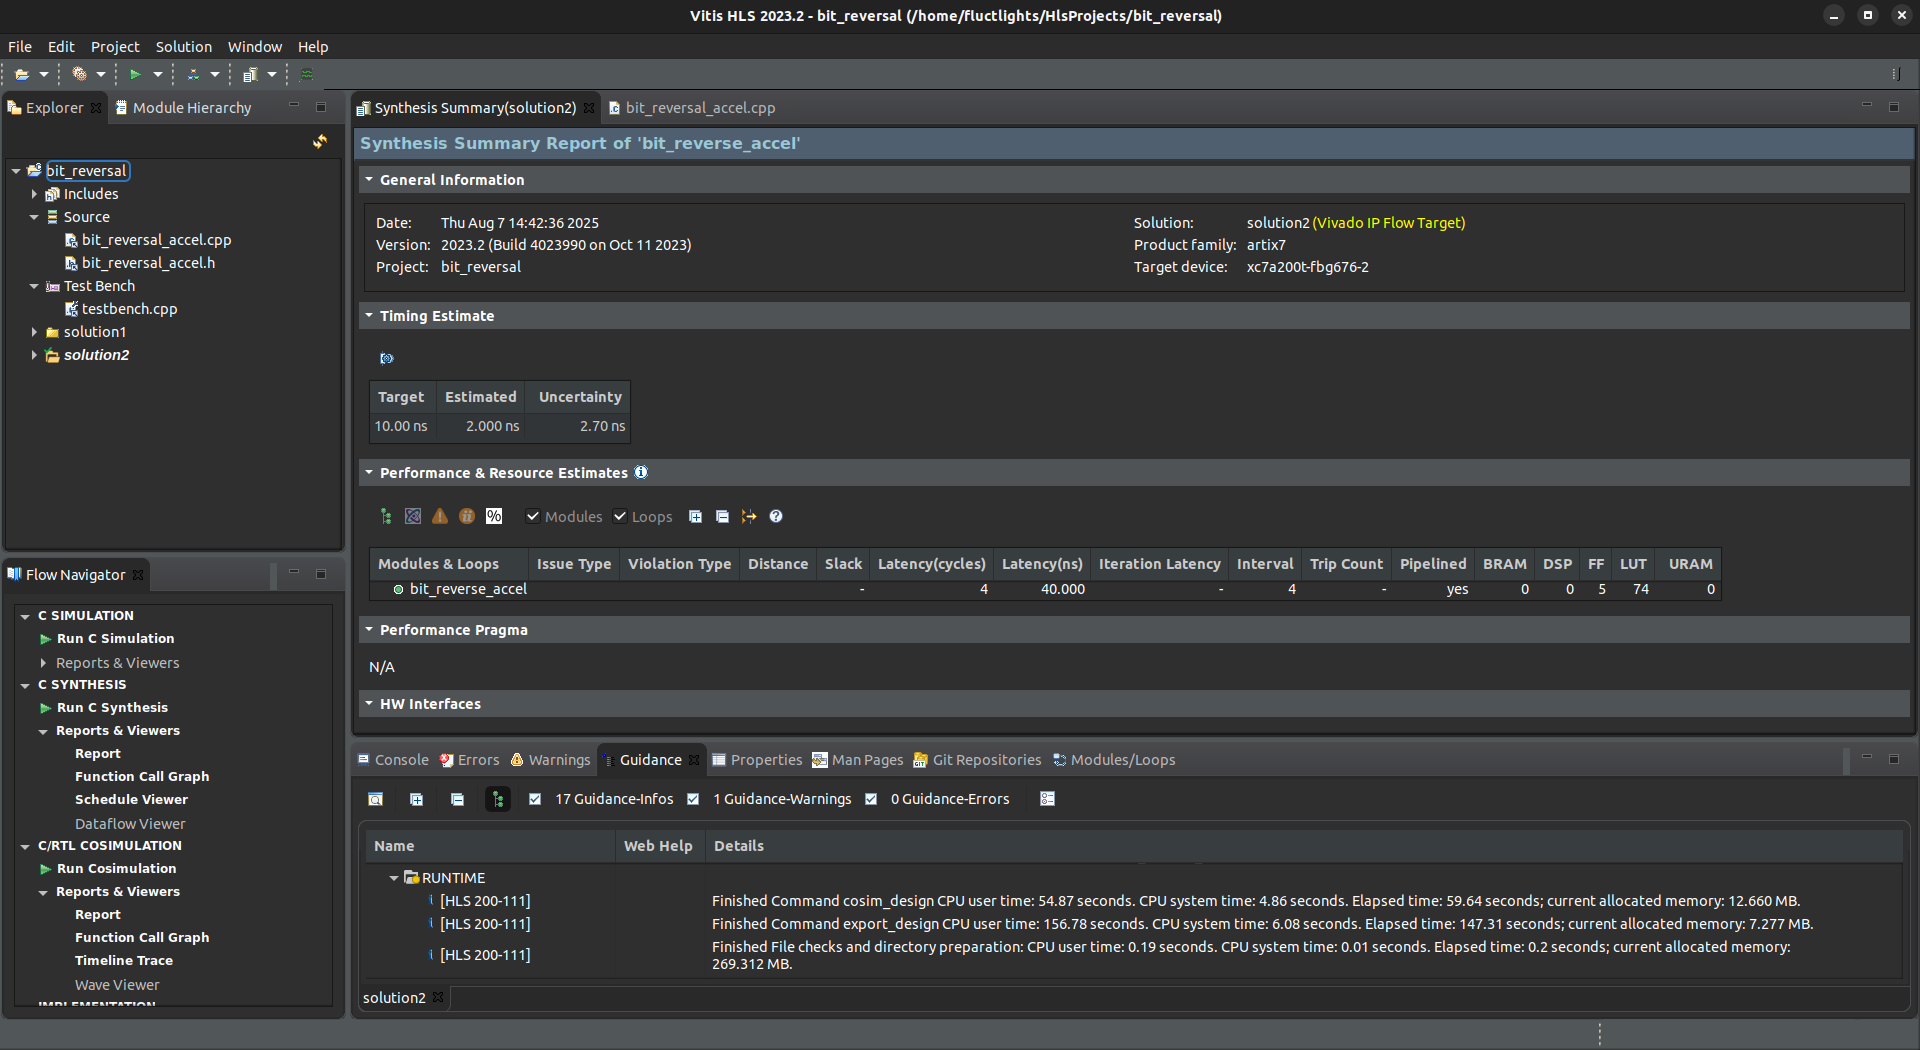
\includegraphics[width=11cm]{figures/proyectoHLS.png}
  \caption{Proyecto abierto}
  \label{fig:proyectoHLS}
\end{figure}

\subsubsection{EdaPlayground}
\label{st:edaplayground}
EDAPlayground es una plataforma en línea gratuita que permite escribir, simular y compartir código de diseño digital utilizando lenguajes de descripción de hardware como Verilog, SystemVerilog y VHDL. Esta herramienta está orientada a estudiantes e ingenieros que quieren realizar simulaciones y compilaciones de diseños hardware sin tener que instalar software especializado. EdaPlayground tiene además, la posibilidad de compartir proyectos fácilmente mediante enlaces, lo convirtiéndolo en una herramienta ideal para tareas de equipo y docencia. Es precisamente por estas cualidades que ha sido la herramienta elegida como alternativa a la Vivado Suite para realizar pruebas de simulación, pudiendo verse el Playground en cuestión \href{https://edaplayground.com/x/tmnc}{en el siguiente enlace}.

La plataforma ofrece un \ac{IDE} web, donde los usuarios pueden crear módulos de diseño y \textit{testbenchs}, además de compilarlos y simularlos utilizando diferentes herramientas de simulación proporcionadas por proveedores como Synopsys. Entre los simuladores disponibles se encuentran ModelSim, o el utilizado en el contexto de este trabajo, QuestaSim, de Siemens, en su versión 2023.2. Además, EdaPlayground permite visualizar resultados de simulación, ya sea en forma de texto EPWave, lo que facilita el análisis del comportamiento del circuito. Sin embargo, debido a la complejidad de la simulación, se ha dependido de otra herramienta de visualización llamada \emph{GTKwave}, explicada posteriormente.

\subsubsection{GTKwave}
\label{st:gtkwave}
GTKwave es un software de visualización de señales de onda, al igual que EPWave de EdaPlayground. Éste es, sin embargo, mucho más potente, pues permite ver un mayor intervalo de tiempo, entre otras cuestiones y al estar instalado en local (es una instalación muy ligera y fácil de instalar con Aptitude) posee una mayor integración con el entorno gráfico del ordenador en cuestión. Para los diagramas de onda de EdaPlayground se ha utilizado GTKWave por su gran ligereza y potencia, así como su fácil usabilidad.

\begin{figure}[!ht]
  \centering
  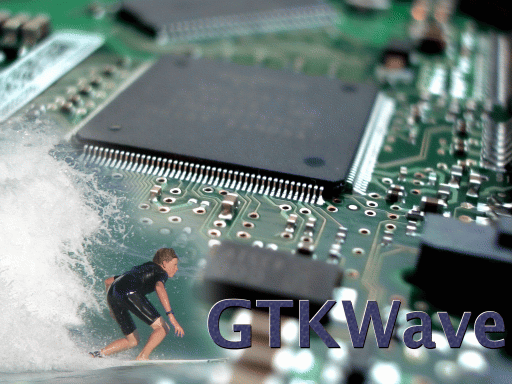
\includegraphics[width=10cm]{figures/gtkwaveLogo.png}
  \caption{Logo de GTKWave}
  \label{fig:gtkwaveLogo}
\end{figure}